\documentclass{standalone}
\usepackage{tikz}
\usetikzlibrary{patterns, positioning}

\begin{document}
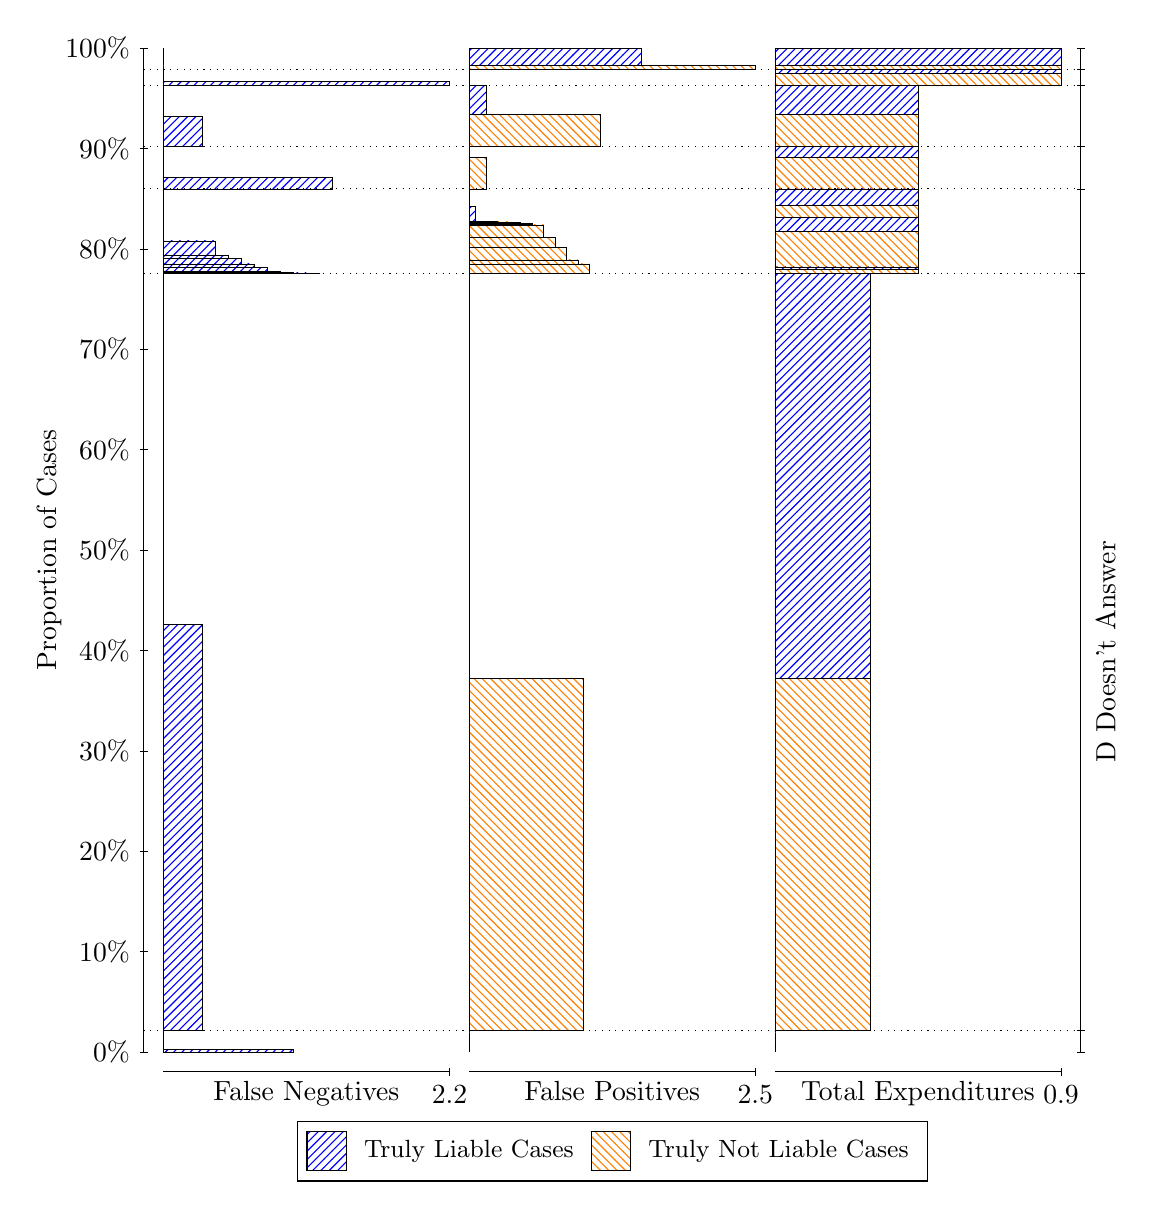
\begin{tikzpicture}
\draw[black, very thin] (1.5,1.75) -- (1.5,14.5);
\node[rotate=90, anchor=center] at (0.3, 8.125) {Proportion of Cases};
\draw[black, very thin] (1.45,1.75) -- (1.55,1.75);
\node[anchor=east] at (1.45, 1.75) {0\%};
\draw[black, very thin] (1.45,3.025) -- (1.55,3.025);
\node[anchor=east] at (1.45, 3.025) {10\%};
\draw[black, very thin] (1.45,4.3) -- (1.55,4.3);
\node[anchor=east] at (1.45, 4.3) {20\%};
\draw[black, very thin] (1.45,5.575) -- (1.55,5.575);
\node[anchor=east] at (1.45, 5.575) {30\%};
\draw[black, very thin] (1.45,6.85) -- (1.55,6.85);
\node[anchor=east] at (1.45, 6.85) {40\%};
\draw[black, very thin] (1.45,8.125) -- (1.55,8.125);
\node[anchor=east] at (1.45, 8.125) {50\%};
\draw[black, very thin] (1.45,9.4) -- (1.55,9.4);
\node[anchor=east] at (1.45, 9.4) {60\%};
\draw[black, very thin] (1.45,10.675) -- (1.55,10.675);
\node[anchor=east] at (1.45, 10.675) {70\%};
\draw[black, very thin] (1.45,11.95) -- (1.55,11.95);
\node[anchor=east] at (1.45, 11.95) {80\%};
\draw[black, very thin] (1.45,13.225) -- (1.55,13.225);
\node[anchor=east] at (1.45, 13.225) {90\%};
\draw[black, very thin] (1.45,14.5) -- (1.55,14.5);
\node[anchor=east] at (1.45, 14.5) {100\%};

\draw[black, very thin] (13.4,1.75) -- (13.4,14.5);
\draw[black, very thin] (13.35,1.75) -- (13.45,1.75);
\node[anchor=west] at (13.35, 1.75) {};
\draw[black, very thin] (13.35,2.027) -- (13.45,2.027);
\node[anchor=west] at (13.35, 2.027) {};
\draw[black, very thin] (13.35,11.638) -- (13.45,11.638);
\node[anchor=west] at (13.35, 11.638) {};
\draw[black, very thin] (13.35,12.712) -- (13.45,12.712);
\node[anchor=west] at (13.35, 12.712) {};
\draw[black, very thin] (13.35,13.255) -- (13.45,13.255);
\node[anchor=west] at (13.35, 13.255) {};
\draw[black, very thin] (13.35,14.027) -- (13.45,14.027);
\node[anchor=west] at (13.35, 14.027) {};
\draw[black, very thin] (13.35,14.231) -- (13.45,14.231);
\node[anchor=west] at (13.35, 14.231) {};
\draw[black, very thin] (13.35,14.5) -- (13.45,14.5);
\node[anchor=west] at (13.35, 14.5) {};

\draw[black, very thin, pattern color=blue, pattern=north east lines] (1.75,1.75) rectangle (3.4015,1.7791);
\draw[black, very thin, pattern color=orange, pattern=north west lines] (1.75,1.7791) rectangle (1.75,2.027);
\draw[black, very thin, pattern color=blue, pattern=north east lines] (1.75,2.027) rectangle (2.2455,7.1754);
\draw[black, very thin, pattern color=orange, pattern=north west lines] (1.75,7.1754) rectangle (1.75,11.638);
\draw[black, very thin, pattern color=blue, pattern=north east lines] (1.75,11.638) rectangle (3.7318,11.641);
\draw[black, very thin, pattern color=blue, pattern=north east lines] (1.75,11.641) rectangle (3.5667,11.644);
\draw[black, very thin, pattern color=blue, pattern=north east lines] (1.75,11.644) rectangle (3.4015,11.652);
\draw[black, very thin, pattern color=blue, pattern=north east lines] (1.75,11.652) rectangle (3.2364,11.655);
\draw[black, very thin, pattern color=blue, pattern=north east lines] (1.75,11.655) rectangle (3.2364,11.659);
\draw[black, very thin, pattern color=blue, pattern=north east lines] (1.75,11.659) rectangle (3.0712,11.713);
\draw[black, very thin, pattern color=blue, pattern=north east lines] (1.75,11.713) rectangle (2.9061,11.759);
\draw[black, very thin, pattern color=blue, pattern=north east lines] (1.75,11.759) rectangle (2.7409,11.831);
\draw[black, very thin, pattern color=blue, pattern=north east lines] (1.75,11.831) rectangle (2.5758,11.864);
\draw[black, very thin, pattern color=blue, pattern=north east lines] (1.75,11.864) rectangle (2.4106,12.052);
\draw[black, very thin, pattern color=orange, pattern=north west lines] (1.75,12.052) rectangle (1.75,12.712);
\draw[black, very thin, pattern color=blue, pattern=north east lines] (1.75,12.712) rectangle (3.897,12.855);
\draw[black, very thin, pattern color=orange, pattern=north west lines] (1.75,12.855) rectangle (1.75,13.255);
\draw[black, very thin, pattern color=blue, pattern=north east lines] (1.75,13.255) rectangle (2.2455,13.628);
\draw[black, very thin, pattern color=orange, pattern=north west lines] (1.75,13.628) rectangle (1.75,14.027);
\draw[black, very thin, pattern color=blue, pattern=north east lines] (1.75,14.027) rectangle (5.3833,14.076);
\draw[black, very thin, pattern color=orange, pattern=north west lines] (1.75,14.076) rectangle (1.75,14.231);
\draw[black, very thin, pattern color=orange, pattern=north west lines] (1.75,14.231) rectangle (1.75,14.28);
\draw[black, very thin, pattern color=blue, pattern=north east lines] (1.75,14.28) rectangle (1.75,14.5);
\draw[black, very thin, pattern color=orange, pattern=north west lines] (5.6333,1.75) rectangle (5.6333,1.9979);
\draw[black, very thin, pattern color=blue, pattern=north east lines] (5.6333,1.9979) rectangle (5.6333,2.027);
\draw[black, very thin, pattern color=orange, pattern=north west lines] (5.6333,2.027) rectangle (7.0867,6.49);
\draw[black, very thin, pattern color=blue, pattern=north east lines] (5.6333,6.49) rectangle (5.6333,11.638);
\draw[black, very thin, pattern color=orange, pattern=north west lines] (5.6333,11.638) rectangle (7.1593,11.759);
\draw[black, very thin, pattern color=orange, pattern=north west lines] (5.6333,11.759) rectangle (7.014,11.808);
\draw[black, very thin, pattern color=orange, pattern=north west lines] (5.6333,11.808) rectangle (6.8687,11.964);
\draw[black, very thin, pattern color=orange, pattern=north west lines] (5.6333,11.964) rectangle (6.7233,12.094);
\draw[black, very thin, pattern color=orange, pattern=north west lines] (5.6333,12.094) rectangle (6.578,12.253);
\draw[black, very thin, pattern color=orange, pattern=north west lines] (5.6333,12.253) rectangle (6.4327,12.262);
\draw[black, very thin, pattern color=orange, pattern=north west lines] (5.6333,12.262) rectangle (6.4327,12.27);
\draw[black, very thin, pattern color=orange, pattern=north west lines] (5.6333,12.27) rectangle (6.2873,12.285);
\draw[black, very thin, pattern color=orange, pattern=north west lines] (5.6333,12.285) rectangle (6.142,12.292);
\draw[black, very thin, pattern color=orange, pattern=north west lines] (5.6333,12.292) rectangle (5.9967,12.298);
\draw[black, very thin, pattern color=blue, pattern=north east lines] (5.6333,12.298) rectangle (5.706,12.486);
\draw[black, very thin, pattern color=blue, pattern=north east lines] (5.6333,12.486) rectangle (5.6333,12.712);
\draw[black, very thin, pattern color=orange, pattern=north west lines] (5.6333,12.712) rectangle (5.8513,13.113);
\draw[black, very thin, pattern color=blue, pattern=north east lines] (5.6333,13.113) rectangle (5.6333,13.255);
\draw[black, very thin, pattern color=orange, pattern=north west lines] (5.6333,13.255) rectangle (7.3047,13.655);
\draw[black, very thin, pattern color=blue, pattern=north east lines] (5.6333,13.655) rectangle (5.8513,14.027);
\draw[black, very thin, pattern color=orange, pattern=north west lines] (5.6333,14.027) rectangle (5.6333,14.182);
\draw[black, very thin, pattern color=blue, pattern=north east lines] (5.6333,14.182) rectangle (5.6333,14.231);
\draw[black, very thin, pattern color=orange, pattern=north west lines] (5.6333,14.231) rectangle (9.2667,14.28);
\draw[black, very thin, pattern color=blue, pattern=north east lines] (5.6333,14.28) rectangle (7.8133,14.5);
\draw[black, very thin, pattern color=orange, pattern=north west lines] (9.5167,1.75) rectangle (9.5167,1.9979);
\draw[black, very thin, pattern color=blue, pattern=north east lines] (9.5167,1.9979) rectangle (9.5167,2.027);
\draw[black, very thin, pattern color=orange, pattern=north west lines] (9.5167,2.027) rectangle (10.728,6.49);
\draw[black, very thin, pattern color=blue, pattern=north east lines] (9.5167,6.49) rectangle (10.728,11.638);
\draw[black, very thin, pattern color=orange, pattern=north west lines] (9.5167,11.638) rectangle (11.333,11.687);
\draw[black, very thin, pattern color=blue, pattern=north east lines] (9.5167,11.687) rectangle (11.333,11.72);
\draw[black, very thin, pattern color=orange, pattern=north west lines] (9.5167,11.72) rectangle (11.333,12.175);
\draw[black, very thin, pattern color=blue, pattern=north east lines] (9.5167,12.175) rectangle (11.333,12.351);
\draw[black, very thin, pattern color=orange, pattern=north west lines] (9.5167,12.351) rectangle (11.333,12.508);
\draw[black, very thin, pattern color=blue, pattern=north east lines] (9.5167,12.508) rectangle (11.333,12.712);
\draw[black, very thin, pattern color=orange, pattern=north west lines] (9.5167,12.712) rectangle (11.333,13.113);
\draw[black, very thin, pattern color=blue, pattern=north east lines] (9.5167,13.113) rectangle (11.333,13.255);
\draw[black, very thin, pattern color=orange, pattern=north west lines] (9.5167,13.255) rectangle (11.333,13.655);
\draw[black, very thin, pattern color=blue, pattern=north east lines] (9.5167,13.655) rectangle (11.333,14.027);
\draw[black, very thin, pattern color=orange, pattern=north west lines] (9.5167,14.027) rectangle (13.15,14.182);
\draw[black, very thin, pattern color=blue, pattern=north east lines] (9.5167,14.182) rectangle (13.15,14.231);
\draw[black, very thin, pattern color=orange, pattern=north west lines] (9.5167,14.231) rectangle (13.15,14.28);
\draw[black, very thin, pattern color=blue, pattern=north east lines] (9.5167,14.28) rectangle (13.15,14.5);
\draw[black, dotted] (1.5,2.027) -- (13.4,2.027);
\draw[black, dotted] (1.5,11.638) -- (13.4,11.638);
\draw[black, dotted] (1.5,12.712) -- (13.4,12.712);
\draw[black, dotted] (1.5,13.255) -- (13.4,13.255);
\draw[black, dotted] (1.5,14.027) -- (13.4,14.027);
\draw[black, dotted] (1.5,14.231) -- (13.4,14.231);
\draw[black, very thin] (1.75,1.5) -- (5.3833,1.5);
\node[anchor=north] at (3.5667, 1.5) {False Negatives};
\draw[black, very thin] (5.3833,1.45) -- (5.3833,1.55);
\node[anchor=north] at (5.3833, 1.45) {2.2};

\draw[black, very thin] (5.6333,1.5) -- (9.2667,1.5);
\node[anchor=north] at (7.45, 1.5) {False Positives};
\draw[black, very thin] (9.2667,1.45) -- (9.2667,1.55);
\node[anchor=north] at (9.2667, 1.45) {2.5};

\draw[black, very thin] (9.5167,1.5) -- (13.15,1.5);
\node[anchor=north] at (11.333, 1.5) {Total Expenditures};
\draw[black, very thin] (13.15,1.45) -- (13.15,1.55);
\node[anchor=north] at (13.15, 1.45) {0.9};


\node[black, centered, rotate=90] at (13.72, 6.8327) {D Doesn't Answer};






\draw (7.449999999999999,1.5) node[draw=none] (baseCoordinate) {};
\begin{scope}[align=center]
        \matrix[scale=0.5, draw=black, below=0.5cm of baseCoordinate, nodes={draw}, column sep=0.1cm]{
            \node[rectangle, draw, minimum width=0.5cm, minimum height=0.5cm, pattern=north east lines, pattern color=blue] {}; &
            \node[draw=none, font=\small] (B) {Truly Liable Cases}; &
            \node[rectangle, draw, minimum width=0.5cm, minimum height=0.5cm, pattern=north west lines, pattern color=orange] {}; &
            \node[draw=none, font=\small] (B) {Truly Not Liable Cases}; \\
            };
\end{scope}

\end{tikzpicture}
\end{document}